%*****************************************************************************************
%*********************************** Second Chapter **************************************
%*****************************************************************************************
\chapter{Low-Cost Robot: Hardware and Software Requirements}
% **************************** Define Graphics Path **************************
\graphicspath{{Chapter2/Figs/}{Chapter2/Figs/}}

    
\vspace{10mm}
\footnotesize {
\begin{flushright}
\textit{
La semplicit\'a \'e l\'ultima sofisticazione.
}\\
Leonardo Da Vinci
\end{flushright}
}
\vspace{10mm}

%----------------------------------------------------------------------
\section{Hardware Requirements}
%----------------------------------------------------------------------
Different educational robots are reviewed in order propose a low-cost robot for {\librER}.
\subsection{A Review of Educational Robots}
According to the Finch Robot which was proposed by a lab at Carnegie Mellon University
\cite{finchrobot2014}, there are five features that are essential
to be considered when one is designing educational robots:
\begin{itemize}[noitemsep,topsep=0pt,parsep=0pt,partopsep=0pt]
 \item Works everywhere;
 \item Rich Interactivity (Programming should be less tedious);
 \item Aesthetically Appealing;
 \item Robust Hardware; and,
 \item Minimal Curricular Changes.
 \end{itemize}
 The Finch Robot hardware includes: light, temperature, and obstacle sensors,
 Accelerometers, Motors, Buzzer, Full-color beak LED, 
 Pen mount for drawing capability and Plugs into USB port (Figure \ref{fig:finch}).
 One of the main advatange of the Finch robot is that use the USB port as a power
device thus there are no batteries to charge and robot behavior can not be affected
by on-board power levels. The Finch Robot cost is \$ 99.00 USD and it has got both 
hardware and software as closed licences.
\begin{figure}[htbp!] 
\centering    
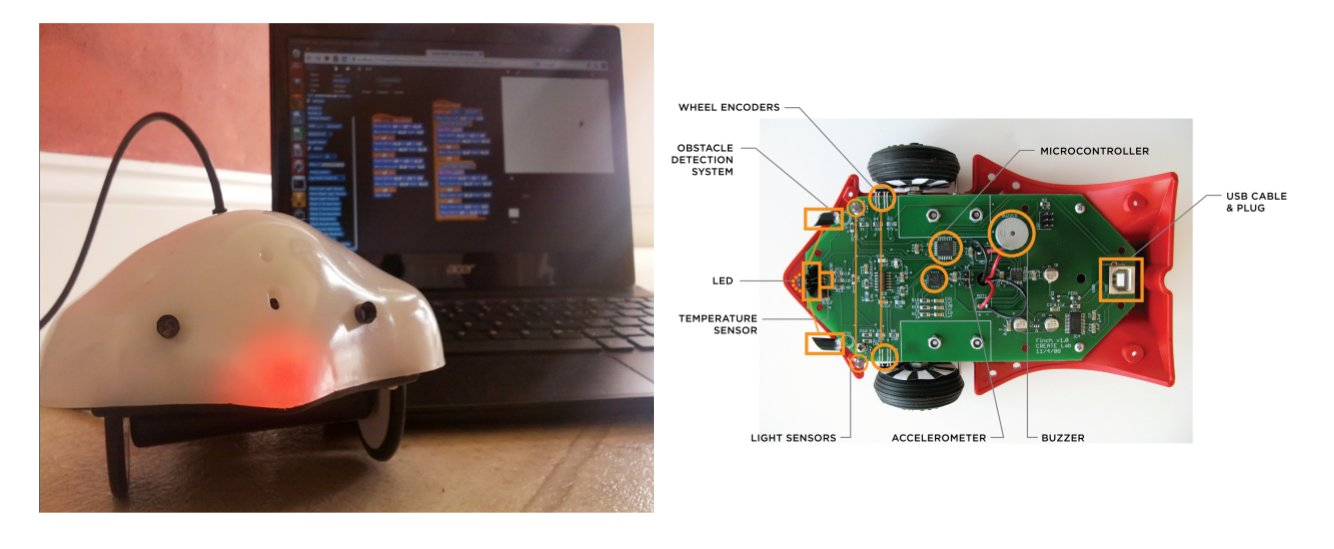
\includegraphics[width=0.9\textwidth]{finch_ps}
\caption[PA]{Finch Robot (left) and Finch' Sensors (right)}
\label{fig:finch}
\end{figure}

Bee-Bot  is a robot designed for use by young children \cite{bee-bot2014}. 
Directional keys are used to enter up to 40 commands which send Bee-Bot forward, back, 
left, and right (Figure \ref{fig:beebot}). Pressing the green GO button starts Bee-Bot 
on its way. Bee-Bot blinks and beeps at the conclusion of each command to allow children 
to follow Bee-Bot through the program they have entered and then confirms its completion 
with lights and sound. Bee-Bot is powered by a built-in rechargeable battery. Recharging 
is done via a standard USB recharger or USB computer port. Bee-Bot cost is \$89.95.
Additionally, a full line of Bee-Bot materials are available to enhance teaching and 
learning with Bee-Bot in the classroom: Bee-Bot lessons \$100.00, problem-solving with 
Bee-Bot \$100.00, and mats from \$29.95 to \$79.95. 
\begin{figure}[htbp!] 
\centering    
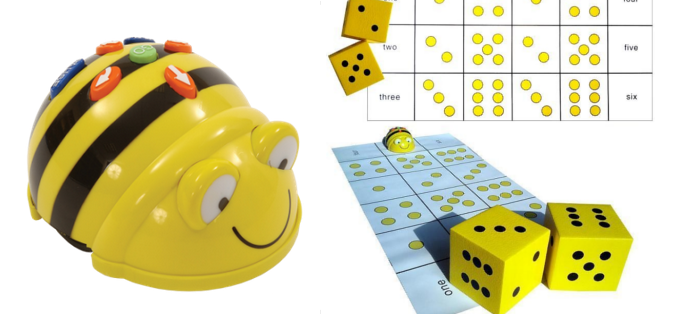
\includegraphics[width=0.5\textwidth]{beebotr}
\caption[PA]{Beebot: Robot (left) and Dice Mat (right).}
\label{fig:beebot}
\end{figure}
 
On the other hand, Thymio II robot is an open hardware and open source project 
\cite{timio}. Thymio II has got over 20 sensors, 40 lights, 2 motors 
(Figure \ref{fig:th}). It occupies a Micro-USB cable for charging and programming.
Thymio II Robot can be used with the integrated behaviours: Friendly (green), Explorer 
(yellow), Fearful (red), Investigator (cyan), Obedient (purple), and Attentive (blue).	
Thymio II Robot can also behave as : Slope avoidance, Balancing on a ball, Musical 
instrument, Light show, Positions in English, Thymio top model, Thymio as a dragon, 
Drawing machine, Learning commands, Special Effects and Light painting. Nonetheless, 
Thymio II's price is \$189 USD which is higher than Finch' Robot cost of \$ 99.00 USD.
\begin{figure}[htbp!] 
\centering    
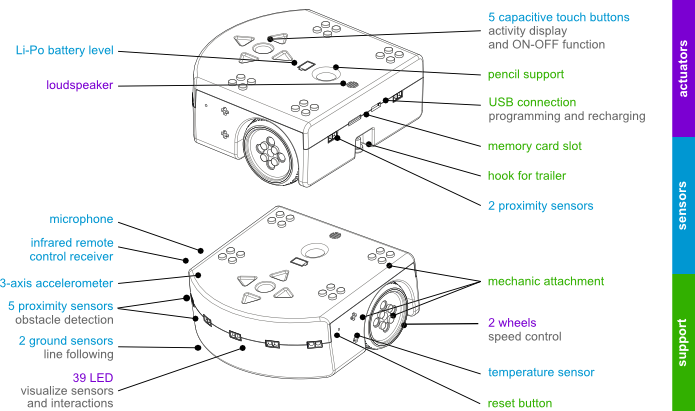
\includegraphics[width=0.6\textwidth]{thymioII-sensor-actuator-color-en}
\caption[PA]{Thymio II Sensor Actuators}
\label{fig:th}
\end{figure}
   

 
Androutsopoulos \emph{et at.}  \cite{Androutsopoulos2014} at the Department of Computer 
Science at Middlesex University from London have designed the MIddlesex Robotic plaTfOrm 
(MIRTO) (Figure. \ref{fig:RacketRobot}) which is an open-source platform built using 
Raspberry Pi, Arduino, and Racket as the core coordination mechanism. Robot's 
hardware has got two platforms: 1) base platform: two HUB-ee wheels with motors and 
encoders (to measure actual rotation), front and rear castors, two bump sensors, an array 
of six infra-red sensors, a rechargeable battery pack, an Arduino microcontroller board;
2) top layer: a Raspberry Pi connected to the Arduino, Linux with Racket (current version 
5.93), USB-WiFi adapter for SSH and network. Additional: cameras, microphones and text to 
speech with speakers. Since it is an educational project, it is not available for being 
bought; however, robot's hardware and software provide a good refeerence.
 \begin{figure}[htbp!] 
\centering    
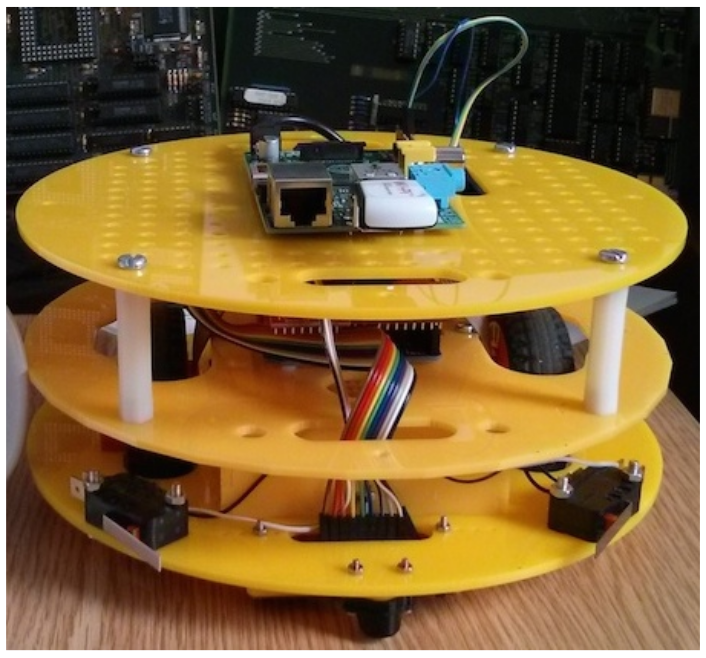
\includegraphics[width=0.4\textwidth]{TheMiddlesexRoboticPlatform}
\caption[PA]{MIddlesex Robotic plaTfOrm (MIRTO)}
\label{fig:RacketRobot}
\end{figure}
 
Equally important, Lil'Bot, a low-cost, open-source, Arduino-compatible balancing robot 
for learning, hacking and delight \cite{lilbot}, is worth to cite since many of its 
features are quite similar to the aim of LibrE Robotics. The main robot characteristics 
are: 1) Arduino Uno compatible; 2) Front, right and left obstable detection using IR 
LEDs; 3) Edge detection using an IR LED; 4) A buzzer plays musical tones and astromech 
droid sounds; 5) Wheel encoders for precise odometry-based control; and 6) the most 
important feature is that Lil' Bot project is released as Open-source hardware and 
software (Left Figure \ref{fig:lilbot}).  More features are shown in Left Figure 
\ref{fig:lilbot}. Lil' Bot can alternatively be energised with an energy source that
is based on Hydrogen Fuel Cells designed by Open Fuel Cell. Lil' Bot is integrated with 
a matrix of LEDs so as to express emotions such as afraid, amused, angry, blissful, 
cool, crying, disappointed, embarrased happy, impatient, naughty, neutral, nonplussed,
outtraged, proud, resigned, sad, sarcastics, shocket, smiling and very sad 
(Right Figure \ref{fig:lilbot}). Since it is a project under development, there is no 
price.
\begin{figure}[htbp!] 
\centering    
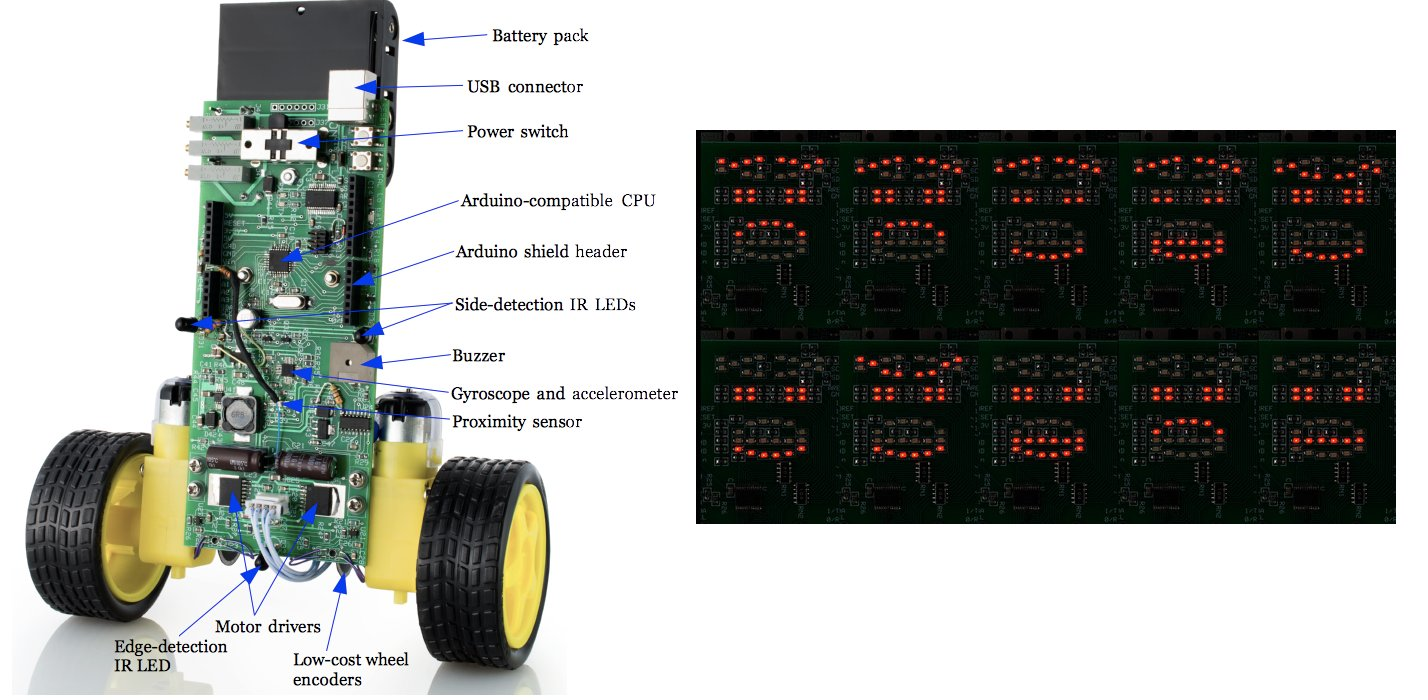
\includegraphics[width=0.8\textwidth]{lilbot}
\caption[PA]{Lil' Bot: Prototype (left), Emotion-like LED display (right)}
\label{fig:lilbot}
\end{figure}

Sparki is an affordable, easy to use, and fun intro to programming, electronics, and 
robotics \cite{sparki}. Sparki is affordable, featured-packed, open-source Arduino robot. 
Sparki comes with a bluetooth module, and array of onboard sensors, precise geared 
stepper motors, a motorized gripper to mention but a few (Figure \ref{fig:sparki}).
Sparki has got the following features: 
1) Ultrasonic distance sensor (get distance from Sparki to walls/objects);
2) 3-Axis Accelerometer (pick-up detection, fall detection, hill climbing);
3) 3-Axis Magnetometer (sense the magnetic field around Sparki, coordinate with 
accelerometer to detect compass heading);
4) Light-sensing phototransistors (light following, darkness seeking);
5) Line-following and edge detection sensors (mazes, line follow, sumo);
6) 128X64 Graphic LCD;
7) RGB LED (RGB = generate any color);
8) Buzzer (beeping, booping, and musical tones);
9) IR Transmitter (like your TV remote control);
10) IR Receiver (like your TV);
11) IR Remote control (lots of buttons to control Sparki with);
12) TTL Serial port for expansion (talk to an Arduino/Raspberry Pi);
13) Bluetooth Serial Module;
14) Powered by 4xAA batteries (not included); and,
15) Geared stepper motors (precise, measured movement down to millimeters/ sub-degrees).
Furthermore, Arcrobotics have develop a module to learn about robotics and to test 
programming capabilities which are available at \cite{sparkisoftware}. Total cost of the 
robot is \$150 USD. Sparki is released as a open-source project; yet, there are no 
further information regarding the Chassis and PDB designs other than basic examples 
of its library.
\begin{figure}[htbp!] 
\centering    
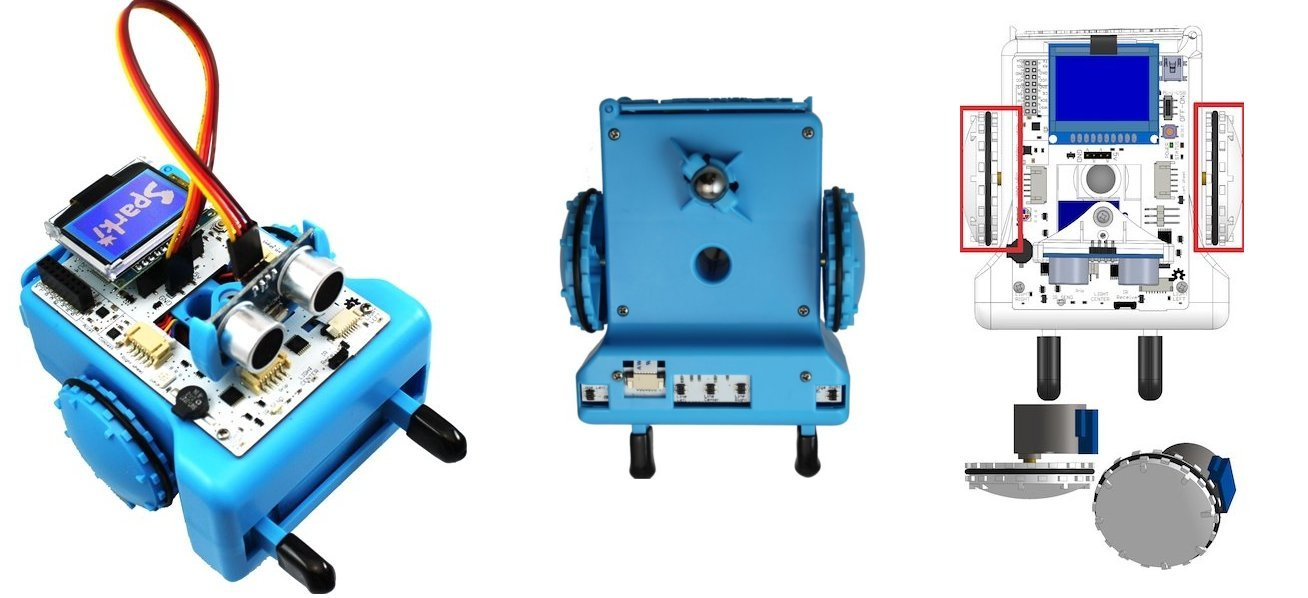
\includegraphics[width=0.7\textwidth]{sparki}
\caption[PA]{Sparki: Prototype (left), bottom part (center) and geared stepper motors 
(right)}
\label{fig:sparki}
\end{figure}
 
 
Mirobot is \textbf{a 100\% open source robot }to which PCB designs and schematics, 
firmware code, and chassis designs are available at \cite{mirobot}. Mirobot uses WiFi 
so that it is easy to get up and running and has been carefully designed to eliminate 
a lot of the difficulties that children  would normally have in building something like 
this (Figure \ref{fig:mirobot}). 
\begin{figure}[htbp!] 
\centering    
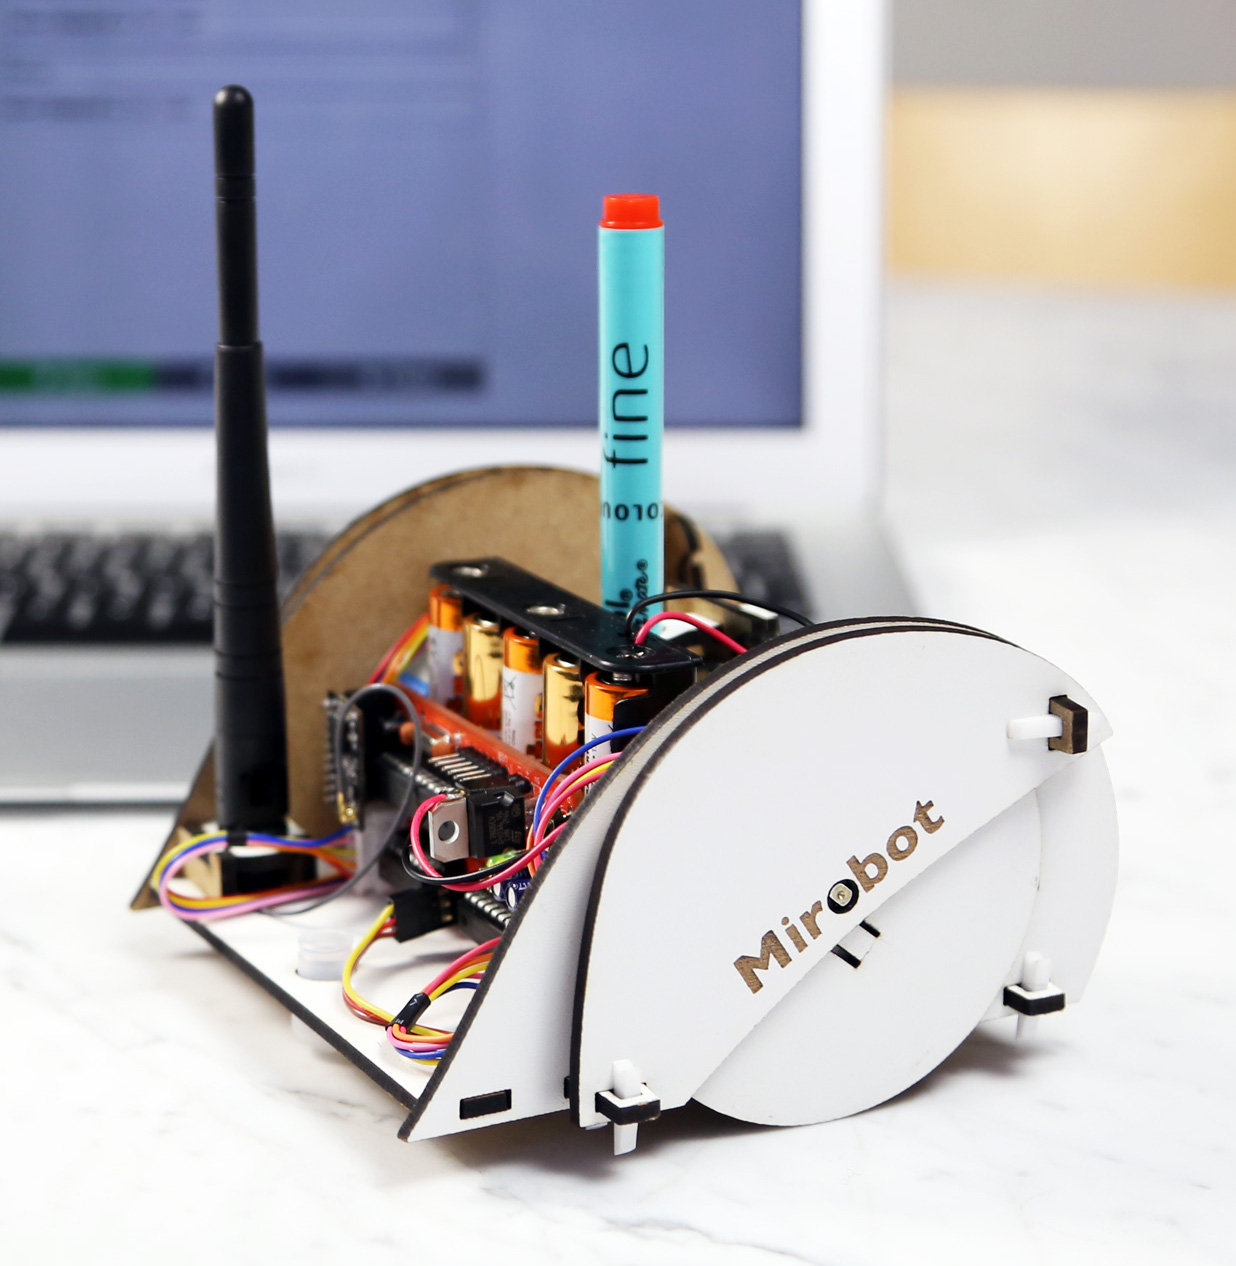
\includegraphics[width=0.5\textwidth]{mirobot}
\caption[PA]{Mirobot}
\label{fig:mirobot}
\end{figure}
 
 
In contrast to the previos-mentioned educational robots, low-cost robots are more 
suitable for the aim of the proyect. For instance, Bug-bot is build with five touch 
sensors, two antennea and three bumbers on 
the back (Figure \ref{fig:bugbot}). It has also got a Xbees wireless board to operate 
the robot with a joystick. Besides, DXF files are available to download in order to be 
easily sent to a laser cutter. PCB diagrams, arduino and processing code is also 
available \cite{bugbot}. 
\begin{figure}[htbp!] 
\centering    
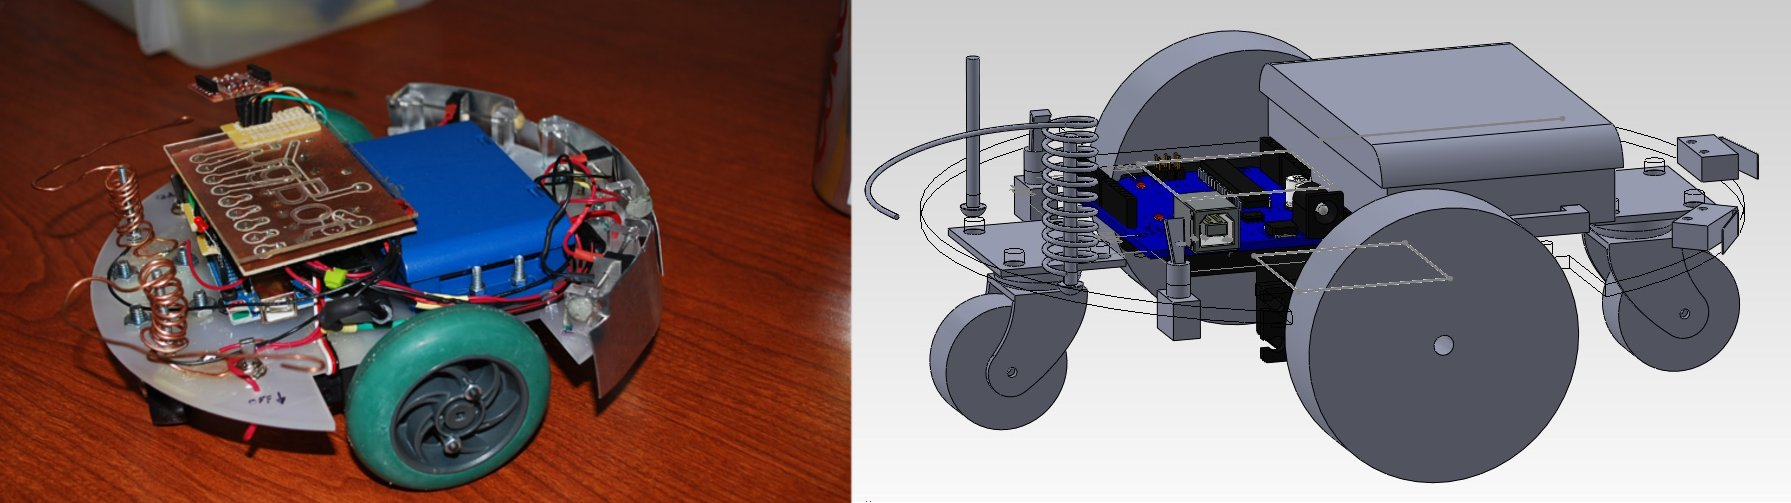
\includegraphics[width=0.75\textwidth]{bugbot}
\caption[PA]{Bug Bot: Prototype (left) CAD layout (right).}
\label{fig:bugbot}
\end{figure}

Boe Bot \cite{boebot}, an arduino line following robot, uses LEDs, light dependent 
resistors (LDRs), an arduino, and a boe bot chassis with 2 continuous rotation servos 
(Figure \ref{fig:boebot}). Nevertheless, the price is not presented in both prototypes.
\begin{figure}[htbp!] 
\centering    
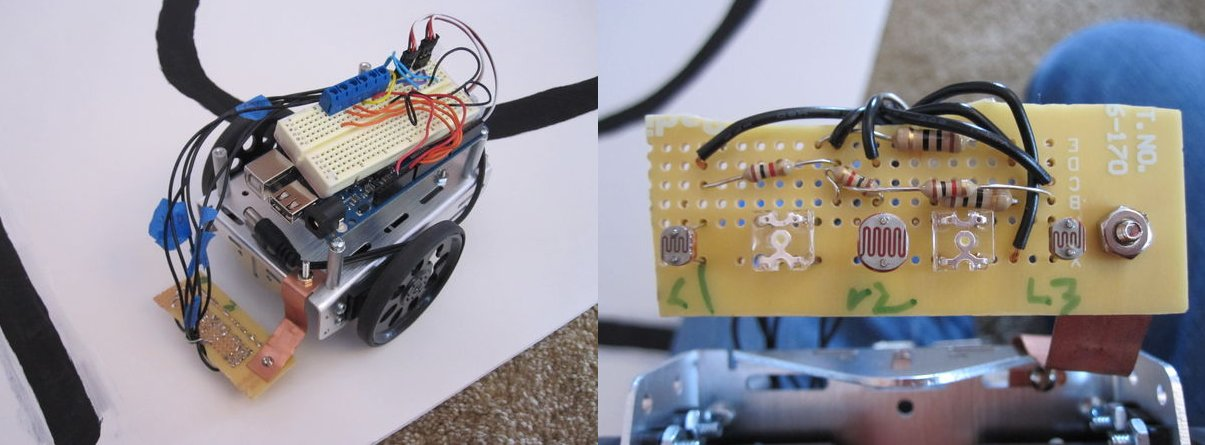
\includegraphics[width=0.7\textwidth]{boebot}
\caption[PA]{Boe Bot: Prototype (left), LDR Sensor Array (right).}
\label{fig:boebot}
\end{figure}
 
Linea is a line follower based on Arduino \cite{linea}. It is build with a robot chassis, 
infrared sensors array, two servo motors and batteries (Figure \ref{fig:linea}). Linea 
uses PID (Proportional-integral-derivative) control to compensate the misalignment from 
the line. The robot use a Pololu sensor with 8 IR leds (14 euros) which has an Arduino 
library (Right figure \ref{fig:linea}). Robot chassis uses a DF robot module (30 euros) 
which offers 2 gear motors, 2 motor sopports and 2 wheels. A motor driver from Sparkfun 
(8 euros), that can feed up to 1.2 Amperes. Others components such as ball caster, sensor 
support, batteries are also used, however, price was not added; henceforth, an estimated 
total price for Linea robot is 55 euros. 
\begin{figure}[htbp!] 
\centering    
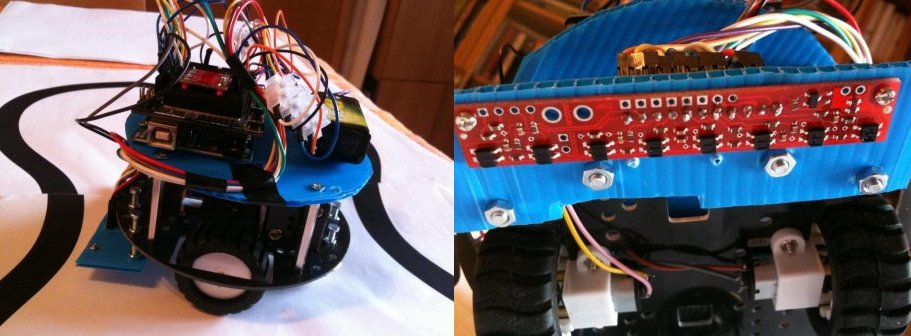
\includegraphics[width=0.6\textwidth]{linea}
\caption[PA]{Linea Robot: Prototype (left), IR Sensor Array (right).}
\label{fig:linea}
\end{figure}

Finally, ArdBot II's design is not an open-source project; nevertheless, it give access 
to the parts list and sources, Construction How-to Manual, Build Your First Robot FAQ,
Where to Get Started sources, and probably the most imporant feature the Print and Cut 
Templates in a zip file  (Rigth Figure \ref{fig:ardbotii}) and Understanding the Build 
Your First Robot Programm \cite{ardbot2}. Chassis material is fairly economical which 
cost \$ 16.95.
\begin{figure}[htbp!] 
\centering    
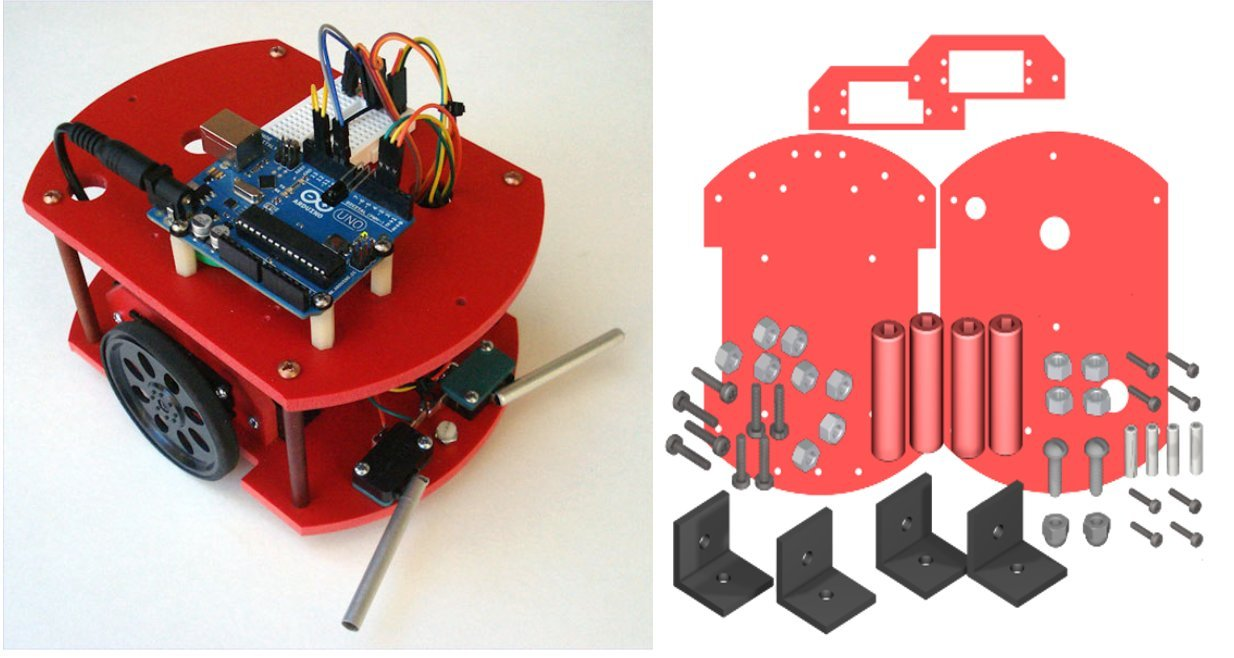
\includegraphics[width=0.6\textwidth]{ardbot2}
\caption[PA]{ArdBot II}
\label{fig:ardbotii}
\end{figure}

%----------------------------------------------------------------------
\subsection{Proposed Low-Cost Robot for {\librER}}

The first proposed low-cost robot for {\librER} is shown in Figure \ref{fig:librerobot}.
It is ensambled by using an Arduino Uno-R3 with the USB port as a power device, two Micro 
Servos TowerPro SG90 that were hacked so as to be a continuous rotation servo 
\cite{servohack1, servohack2}, two wheels (62mm of diametre), two balls caster, two LEDs, 
two LDRs, and four 100KOhms Resistors. The total cost accounts for \$  619 Mexican Pesos 
($\approx$ \$ 48 USD ). From the table \ref{t:lcr}, it can be seen detailed prices for 
the material. 
\begin{figure}[htbp!] 
\centering    
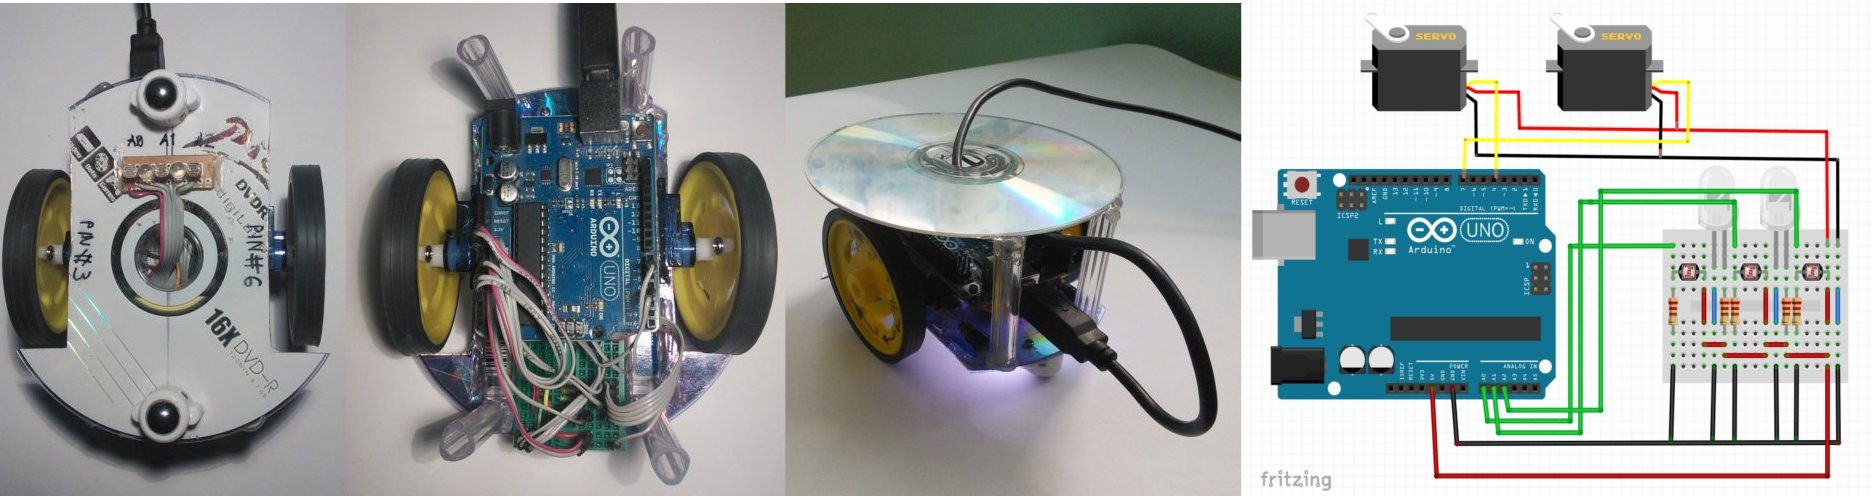
\includegraphics[width=1\textwidth]{librerobot}
\caption[PA]{Proposed Low-cost Robot: Bottom view, top view, front view and
circuit connection (From left to right).}
\label{fig:librerobot}
\end{figure}
It has been thought that total cost can be reduced since material was bought in local 
stores. Additionally, the proposed low-cost robot is under a development stage and, 
it will therefore be evolving according to the possible issues at the testing stage and 
the needs that are considered to be a very low-cost Robot.
 \begin{table}[h]
 \centering
\begin{tabular}
 { l | l }
 \toprule
 
 \textbf{Material} & Price (Mexican Pesos) \\ 
 \midrule
  
 \textbf{Arduino Uno-R3 con cable USB} & \$ 370 \\
 \textbf{2 TowerPro SG90 - Micro Servos} & \$ 160 \\
 \textbf{2 Wheels (62mm of diametre)} &  \$ 38 \\
 \textbf{2 balls caster } & \$ 82 \\
 \textbf{Breadboard - Mini Modular} &  \$ 20 \\
 \textbf{3 LDRs } & \$ 18 \\
 \textbf{2 LEDs } & \$ 10 \\
 \textbf{4 100KOhms Resistors } & \$ 1 \\
 \textbf{Total Cost} & \textbf{\$  699 ($\approx$ \$ 53.86 USD )} \\
 \bottomrule
 \end{tabular}
 \caption{Cost List of the proposed Educational Robot}
\label{t:lcr}
\end{table}
 
Furthermore, two videos were recorded so as to show demo versions of the proposed 
low-cost robot: 1) A Demo Version of the low-cost Robot using Ardublok for {\librER}  
Project, and 2)  A Voice Controlled Low-Cost Robot Using Arduino, 
PocketSphinx \cite{Pocketsphinx}, 
Firmata \cite{DrFirmata}
and Racket \cite{Racket}; 
both can be seen at \url{https://sites.google.com/site/librerobotics/videos}
 
It is worthwhile to mention that some setbacks with the non-linearity of LDR sensors 
have been faced, henceforth the line follower application has not been implemented well;
it is assumed that array sensors will work well with IR sensors. Additionally, 
the hacked servos has been presented an hysteresis behavior since the angles controls 
have a variation of 1 or 2 when sending values to stop the servos and in the case of 
speech recognition, the voice commands are sometimes misrecognized. 
 
%----------------------------------------------------------------------
\section{Software Requirements}
%----------------------------------------------------------------------

\subsection{Arduino}
The Arduino integrated development environment (IDE) is a cross-platform application 
written in Java (Figure \ref{fig:ardublockarduino}), and is derived from the IDE for 
the Processing programming language and the Wiring projects. Arduino IDE includes a code 
editor with features are: syntax highlighting, brace matching, and automatic 
indentation. It is also capable of compiling and uploading programs to the board with 
a single click. A program or code written for Arduino is called a "sketch" \cite{arduino}.

\subsection{Ardublock}
Since {\librER} is aimed to inexperienced users in coding, Ardublock is a suitable tool
which is rooted in blocks that make programming both rich interactive and less tedious. 
Ardublock is a scratch-like programming based on blocks which is reflected by its clear 
transition to text-based coding, it also generates real Arduino code in the background.
Like Arduino, Ardublock is also a run-time Java script.

Ardublock plugin can be downloaded at \cite{ardublock} and the source coude is available 
at \url{https://github.com/taweili/ardublock}. Ardublock Graphical User Interface is 
shown in Figure \ref{fig:ardublockarduino} in which three four parts are illustrated: 
programming blocks palate, zoommed out view, programming area, and arduino code. It also 
presents an example of the configuration of two servo motors that were programming in a 
loop routine of stop, counter clockwise, and clockwise. It is worth to note that settings
for the angle values may differ because of the hacked servo version.

\begin{figure}[htbp!] 
\centering    
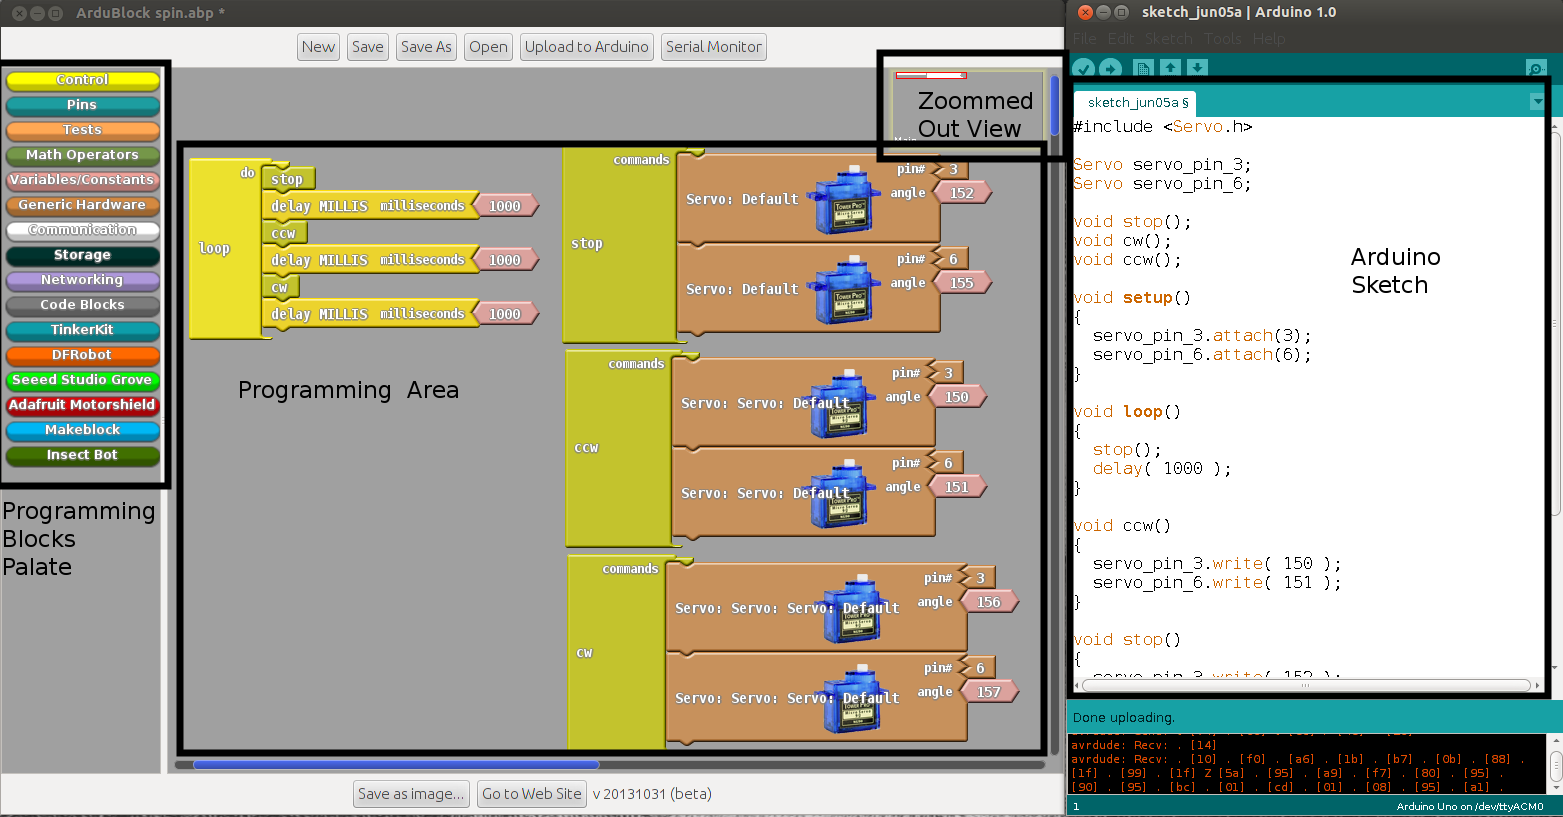
\includegraphics[width=1\textwidth]{ardublockarduino}
\caption[PA]{Examples for Ardublock and Arduino IDE}
\label{fig:ardublockarduino}
\end{figure}
 
